در ابتدا به بررسی پارادایم دیفرانسلی این سوال می‌پردازیم. در اینجا با توجه به تابع تبدیل داریم:

\begin{flalign*}
    \theta(s) &= \frac{Ap}{s(s + p)} \\
    \text{PID}(s) &= \frac{1}{s + 4.54} \\
    \text{Filter}(s) &= \frac{1}{s + 1} 
\end{flalign*}

بنابراین برای طراحی دیاگرام آن نیاز به یک فیلتر،
Grain ،
تابع تبدیل و 
PID
کنترلر داریم. در اینجا سینگال ورودی تابع پله بوده و با استفاده از بلوک
Mux
در
Scope
توانسته‌ایم که سیگنال خروجی را براساس ورودی رسم کنیم. شکل دیاگرام طراحی شده برای این قسمت در پایین قابل مشاهده است.

\vspace{-10pt}

\begin{figure}[h]
    \centering
    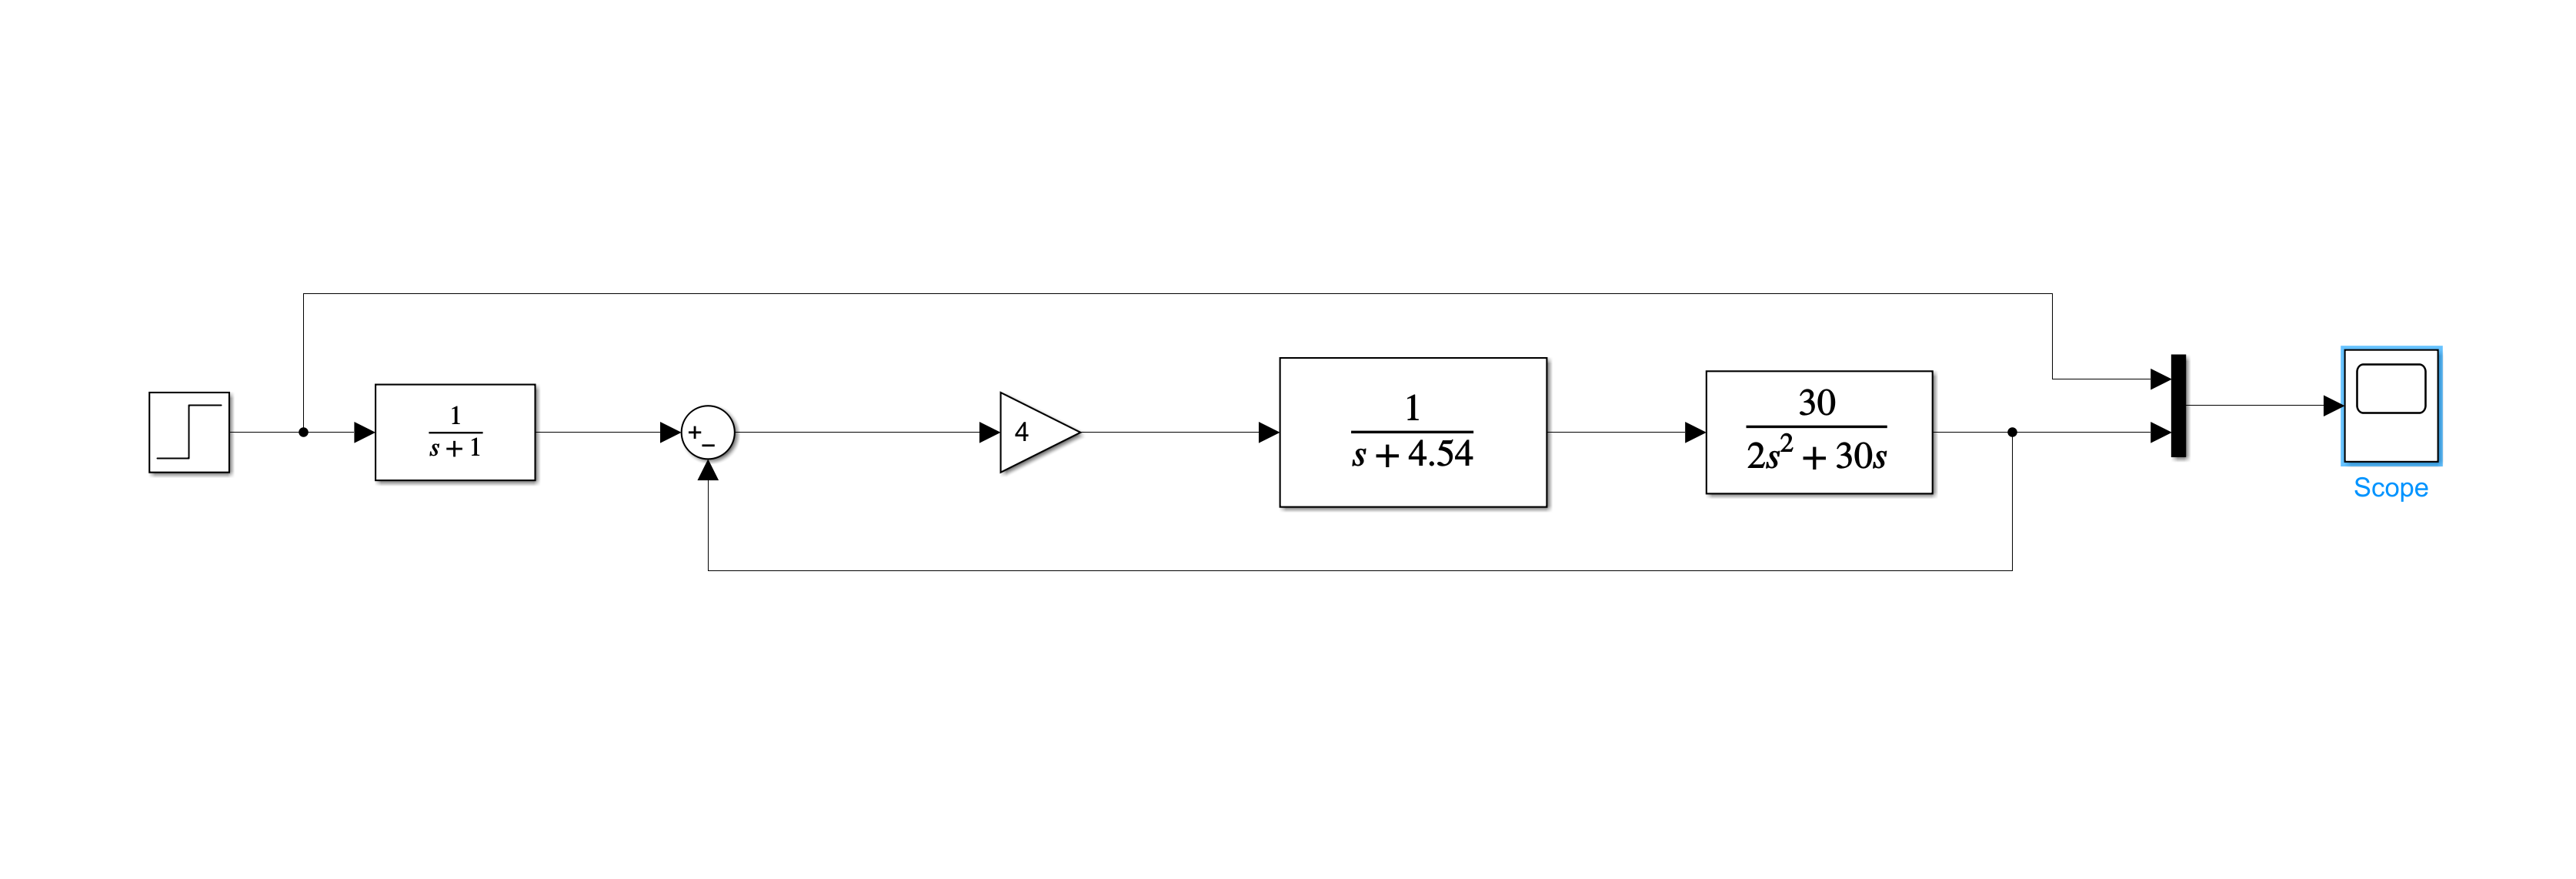
\includegraphics[width = 0.8\textwidth]{commons/image1.png}
    \caption{دیاگرام پارادایم دیفرانسلی}
\end{figure}

همچنین خروجی این پارادایم به این صورت قابل مشاهده است:

\begin{figure}[h]
    \centering
    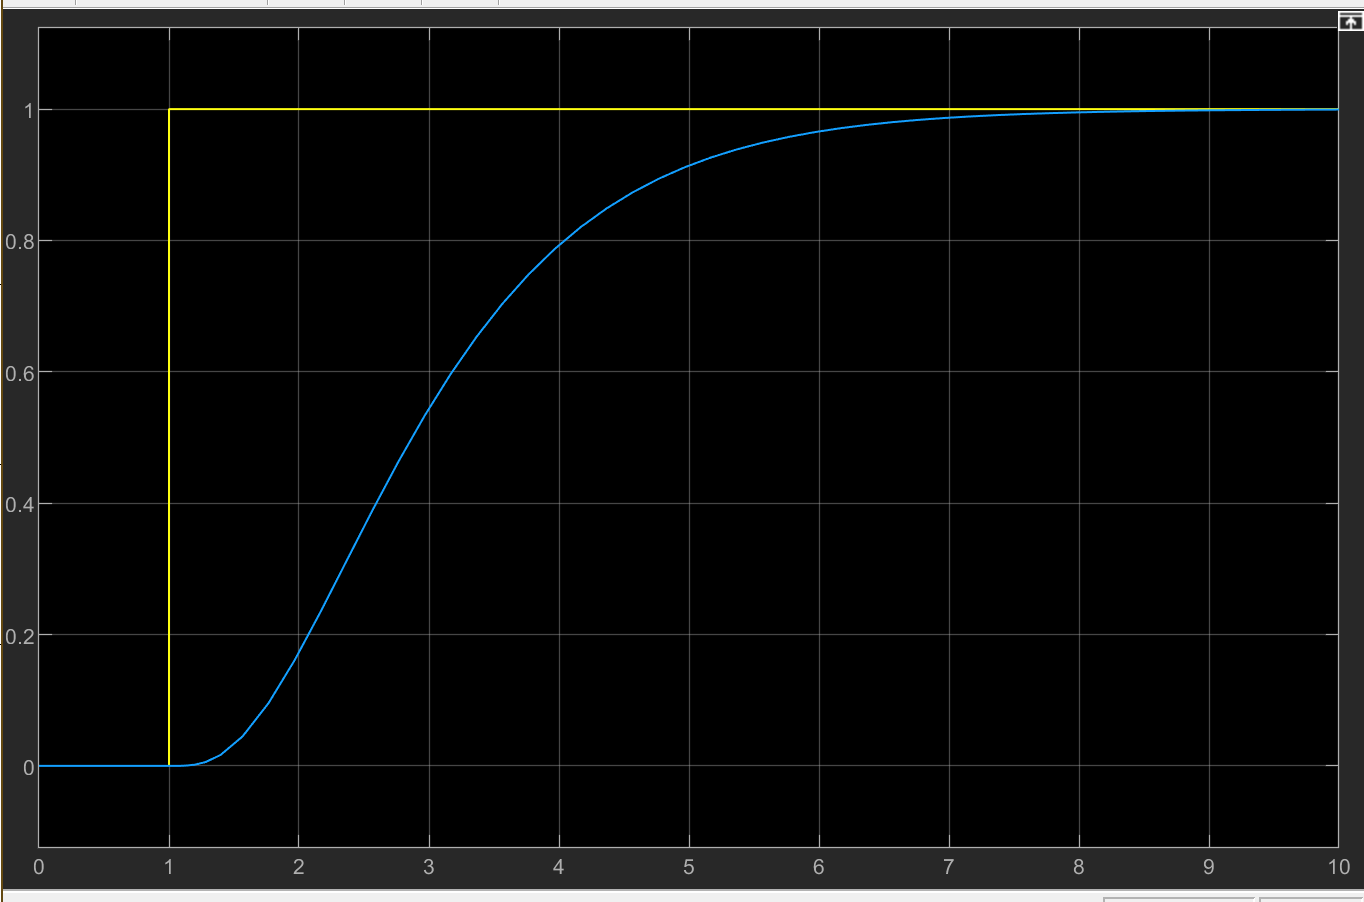
\includegraphics[width = 0.6\textwidth]{commons/image2.png}
    \caption{خروجی پارادایم دیفرانسلی}
\end{figure}

همانطور که در خروجی این قسمت می‌بینیم، سیگنال خروجی به صورت پیوسته در حال تغییر است و پس از دریافت سیگنال پله به عنوان ورودی، پس از مدتی به حالت تعادل خود رسیده است.

در این بخش به طراحی پارادایم
\lr{State Chart}
می‌پردازیم. کاری که باید در اینجا انجام دهیم این است که براساس دما حالت‌های مختلف را ایجاد کنیم و رفتاری گسسته‌وار در مقابل تغییرات دما داشته باشیم.

در اینجا ما دو کامپوننت
Cooler
و
Heater
داریم که براساس شریط 
Tempreture
در حال جابه‌جایی بین استیت‌های مختلف هستند. سینگال ورودی در این سیستم از نوع تابع
\lr{Sinc wave}
بوده و در خروجی شاهد حالات
Cooler
و
Heater
براساس ورودی هستیم.

شکل
\lr{State Flow}
طراحی شده برای این منظور را به این صورت می‌توانید مشاهده کنید:

\begin{figure}[h]
    \centering
    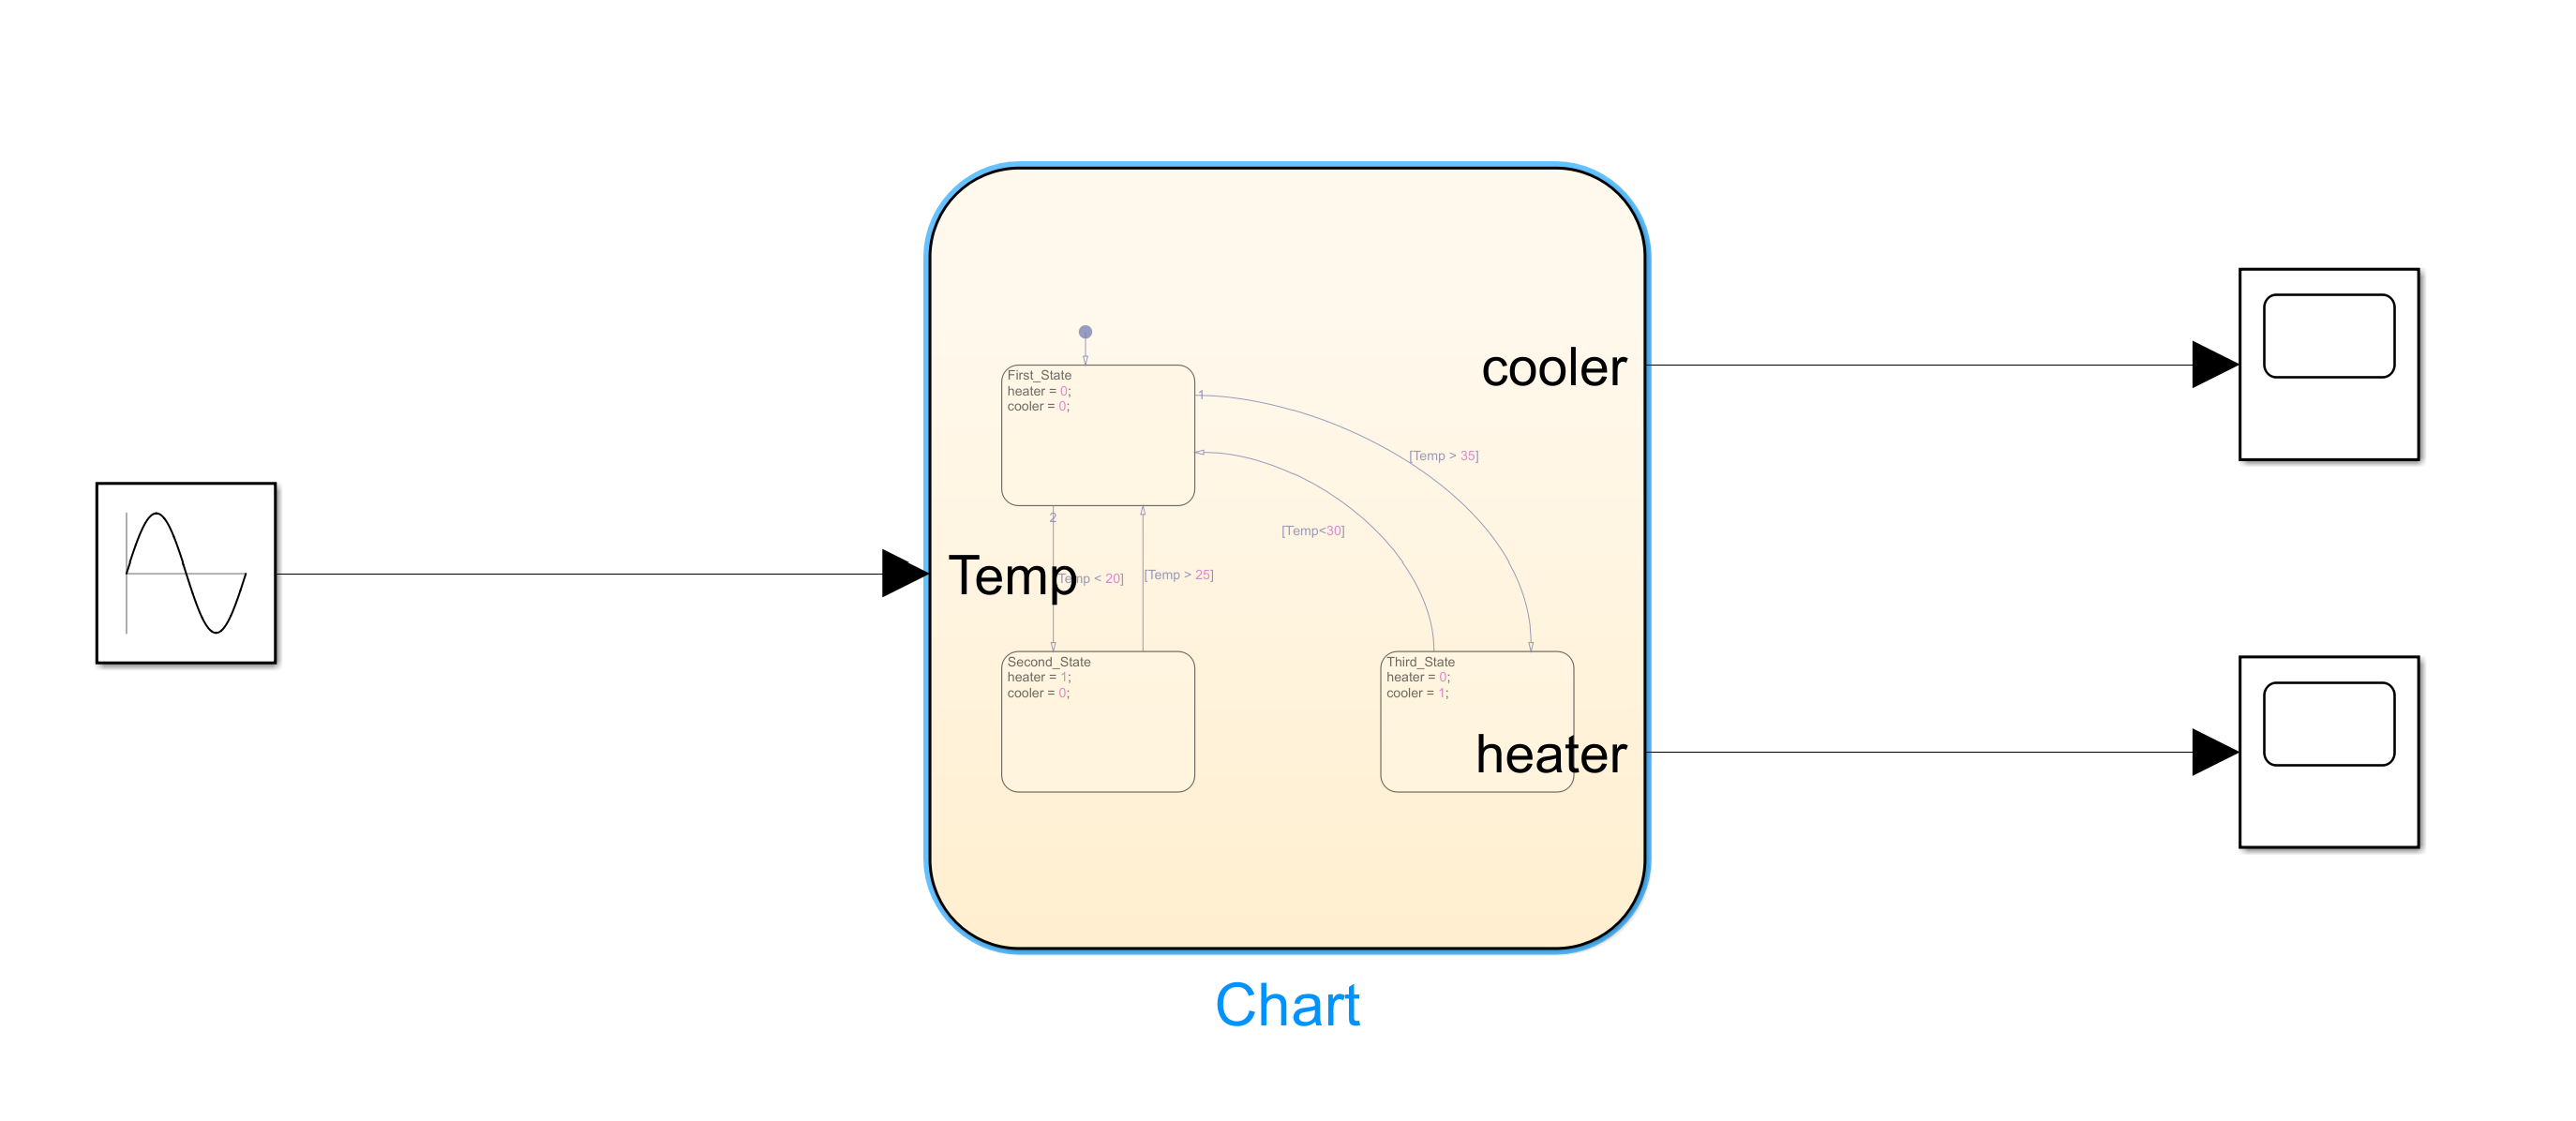
\includegraphics[width = 0.8\textwidth]{commons/image3.png}
    \caption{طراحی استیت‌های سیستم کنترل دما}
\end{figure}

همچنین دیاگرام کلی به این صورت خواهد بود:

\begin{figure}[h]
    \centering
    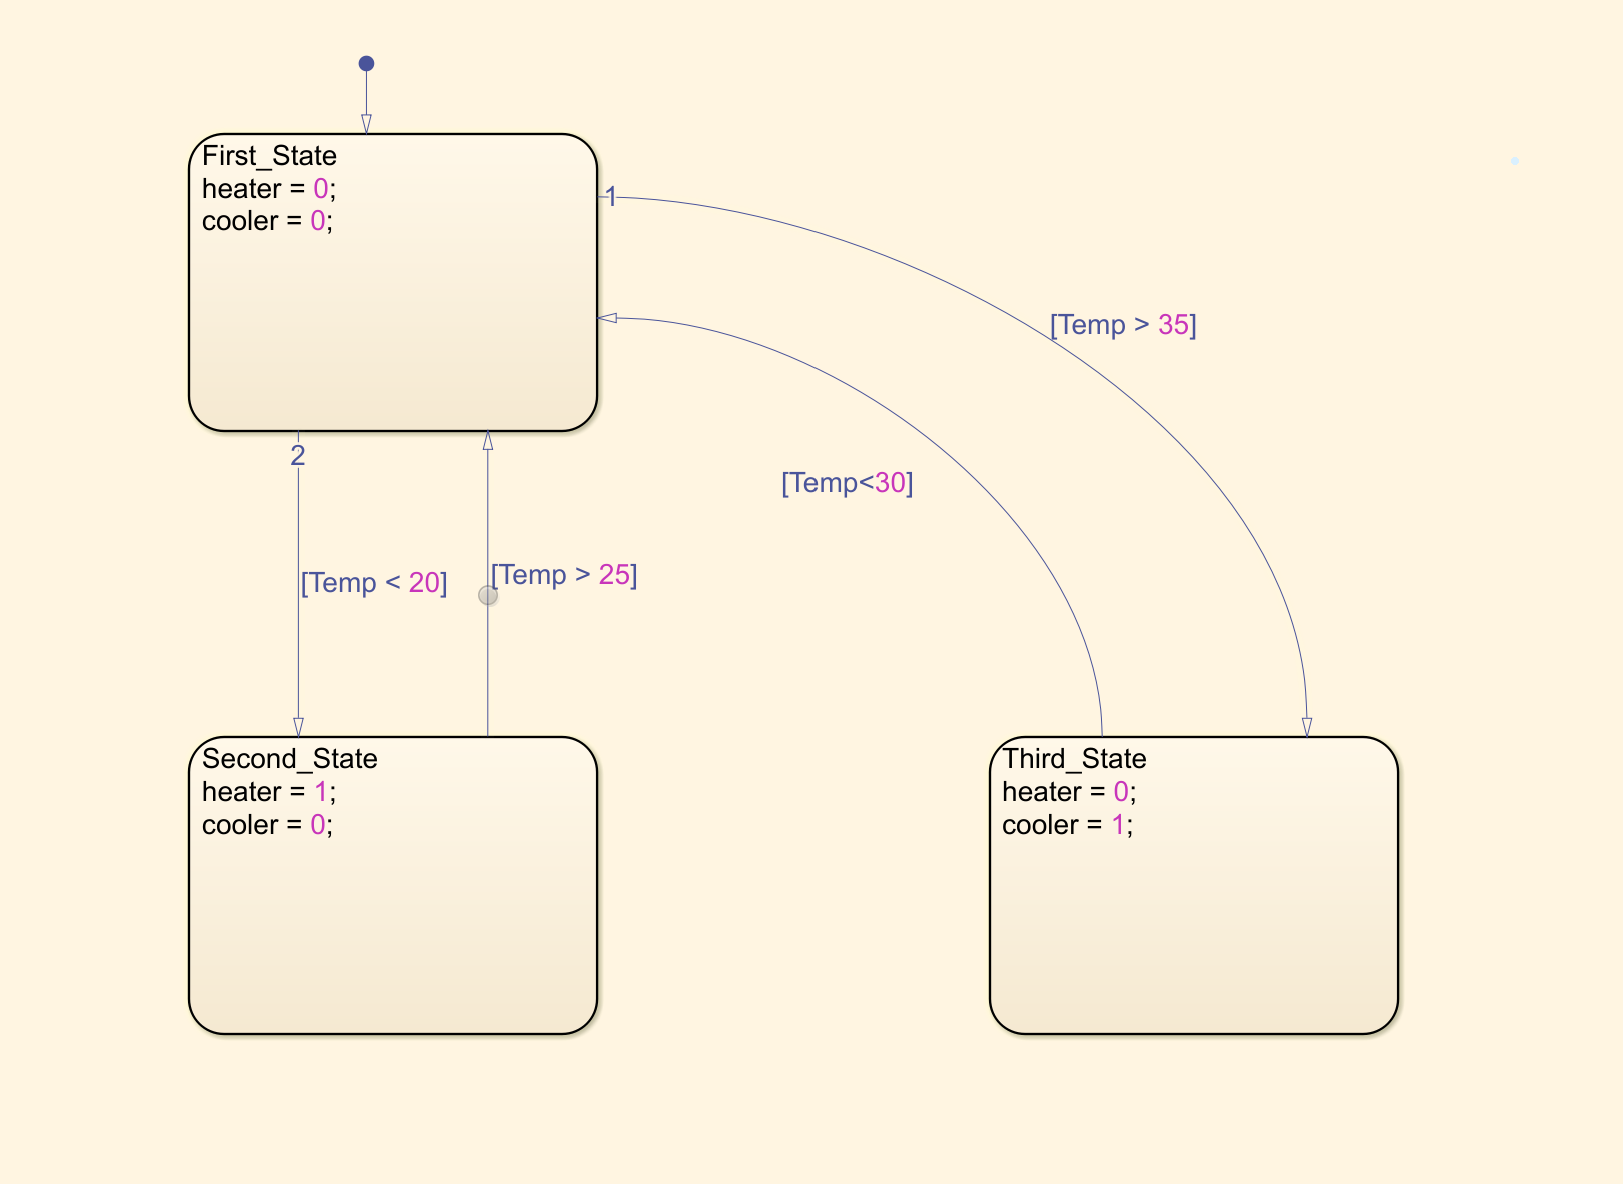
\includegraphics[width = 0.8\textwidth]{commons/image4.png}
    \caption{دیاگرام کلی مدل}
\end{figure}

\newpage

در نهایت برای خروجی‌های
Cooler
و
Heater
خواهیم داشت:

\begin{figure}[h]
    \centering
    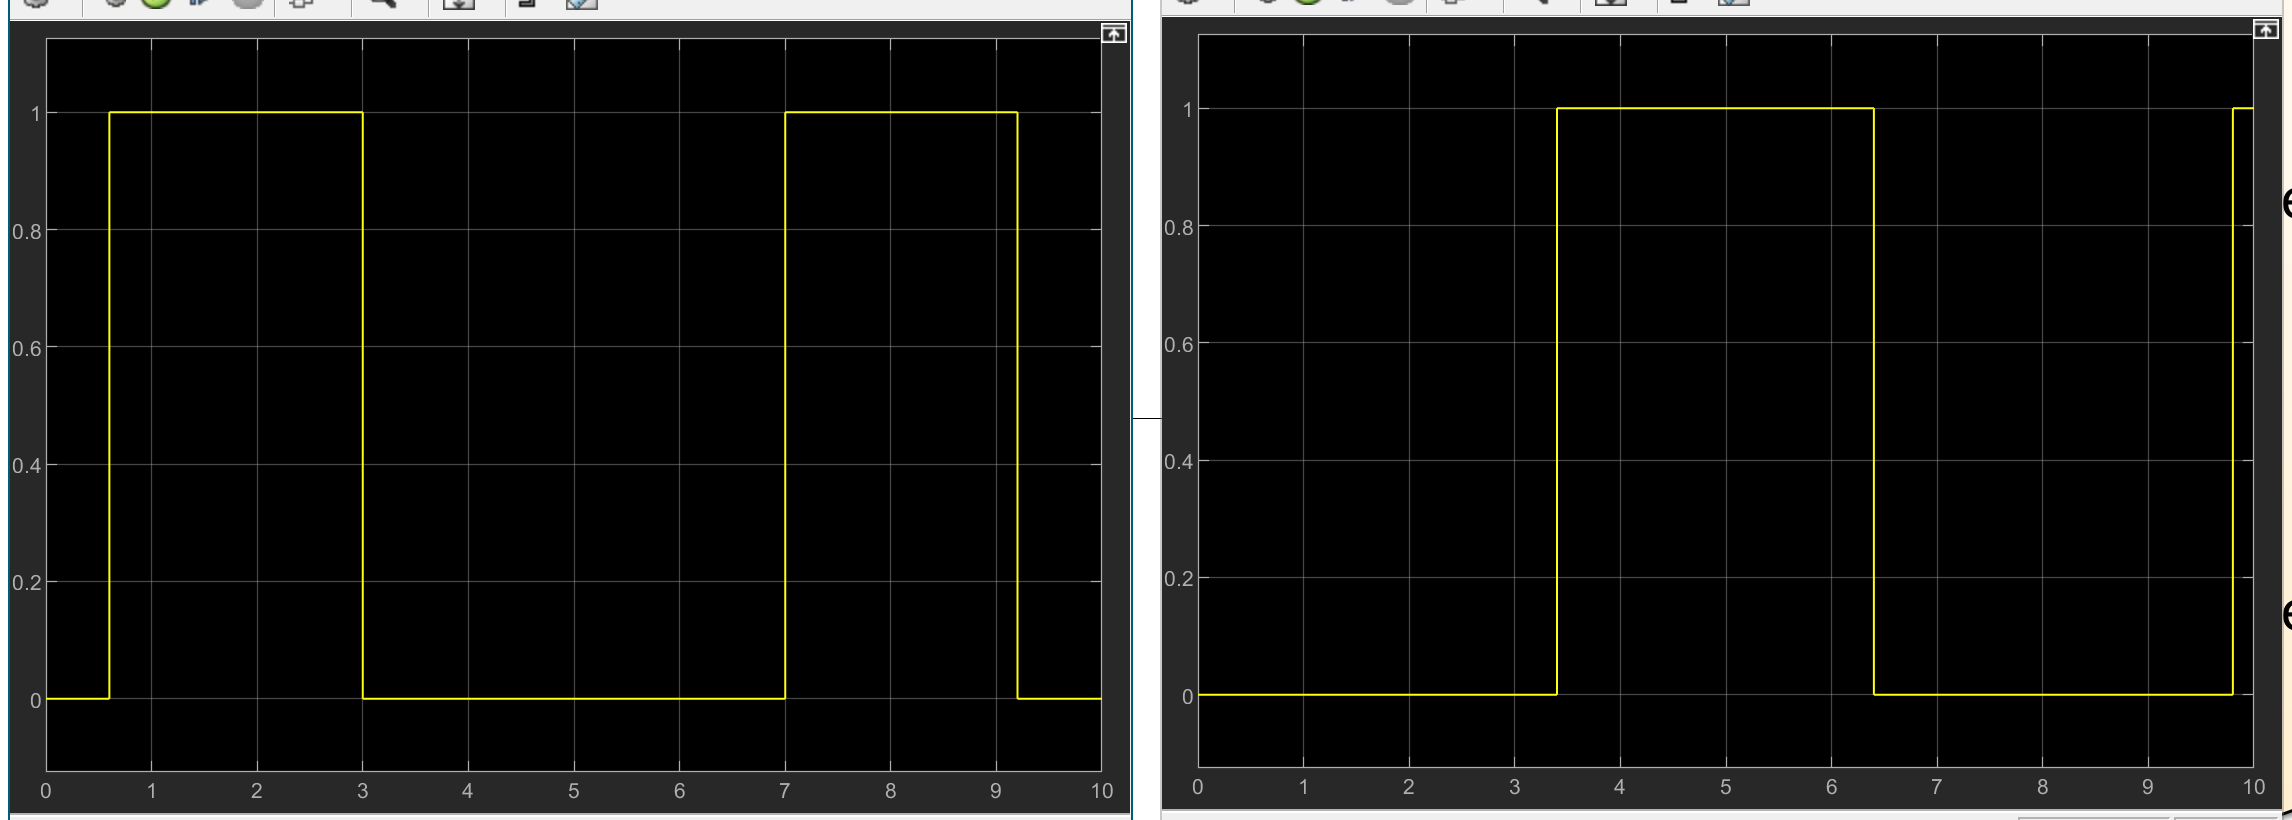
\includegraphics[width = \textwidth]{commons/image5.png}
    \caption{خروجی مدل استیت چارت}
\end{figure}

همانگونه که مشاهده می‌کنید در اینجا براساس ورودی دما یا در حالتی هستیم که 
Heater
روشن بوده یا
Cooler
و یا اینکه هر دو خاموش هستند.

تفاوت اصلی این دو پارادایم در نوع پاسخ سیستم به تغییرات است. در پارادایم براساس معادلات دیفرانسلی ما شاهد این هستیم که سیستم پاسخی پیوسته و همواره در حال تغییر به ورودی ما می‌دهد. در صورتی که در پارادایم استیت چارت خروجی‌های به صورت صفر و یک بوده و صرفا مشخص می‌کند که براساس ورودی داده شده باید در چه حالت‌های از پیش تعیین شده‌ای قرار بگیریم.

به این ترتیب با توجه به نوع سیستمی که در نظر داریم پیاده کنیم و نوع سیگنال ورودی می‌بایست یکی از این دو نوع پارادایم را برای مدل‌سازی سیستم‌مان در نظر بگیریم و هر کدام از پارادایم‌ها کاربرد به خصوص خودشان را خواهند داشت.